\documentclass[17pt, a0paper, margin=0mm, innermargin=5mm, blockverticalspace=5mm, colspace=5mm, subcolspace=-15mm]{tikzposter}
% 594 x 841 mm
\useinnerblockstyle{Table}
\usepackage{fontspec}
% \setmainfont{Charis SIL}
% \setsansfont{Charis SIL Compact}
\setmainfont{DejaVu Serif}
\setsansfont{DejaVu Serif}

\usepackage{enumitem}

% \tikzposterlatexaffectionproofoff

\title{\parbox{\linewidth}{\centering \textsf{Analyzing Uncertainty in Time Series\\Modeling of Hydraulic Heads}}}
\author{\textsf{Martin Vonk$^{1,4}$, Raoul Collenteur$^2$, Jeremy White$^3$ \& Mark Bakker$^4$}}
\institute{\textsf{1: Artesia BV, Schoonhoven, The Netherlands. 2: Eawag, Dübendorf, Switzerland.\\3: Intera, Fort Collins, United States. 4: Delft University of Technology, The Netherlands.}\vspace{-6mm}}


% Davos logo kleuren
% luchtblauw: 5EBFED 
% rotsgrijs: 9D9D9C
% waterblauw: 0077BA
% bodemgrijs: 373736

\newcommand{\colorTitle}{373736}            % title block main color
\newcommand{\colorTitleGradient}{5EBFED}    % title block gradient color
\newcommand{\colorBlockTitle}{5EBFED}       % color of block title
\newcommand{\colorBlock}{C9F1FF}          % color of blocks
% \newcommand{\colorBlock}{F5D491}            % color of blocks
\newcommand{\colorBlockTitleText}{FFFFFF}   % color of block title text

% new color definitions for Desert theme
\definecolorpalette{GrayOrangeBlue}{
    \definecolor{colorOne}{HTML}{\colorTitle} %bovenkant
    \definecolor{colorTwo}{HTML}{\colorBlock} %tekstvakken
    \definecolor{colorThree}{HTML}{\colorBlockTitle} %tekstkoppen
}

\definecolor{gradientcolor}{HTML}{\colorTitleGradient} % bottom color for title block and top color for lower block

% Remove gradient in title block
\definetitlestyle{VerticalShading}{
	width=\paperwidth, roundedcorners=0, linewidth=0pt, innersep=1.5cm,
	titletotopverticalspace=0mm, titletoblockverticalspace=20mm,
	titlegraphictotitledistance=10pt, titletextscale=1
}{
   \draw[draw=none, bottom color=gradientcolor, top color=colorOne]%
   (\titleposleft,\titleposbottom) rectangle (\titleposright,\titlepostop);
}
% remove gradient in bottom (modify top color=...)
\definebackgroundstyle{BottomVerticalGradation}{
	\draw[draw=none, line width=0pt, bottom color=colorOne, 
	    top color=gradientcolor] (bottomleft) rectangle ($(bottomleft)+(\textwidth,3)$); 
}

% remove gradient in text block titles (modify right color=...)
\defineblockstyle{Slide}{
	titlewidthscale=1, bodywidthscale=1, titleleft,
	titleoffsetx=0pt, titleoffsety=0pt, bodyoffsetx=0pt, bodyoffsety=0pt,
	bodyverticalshift=0pt, roundedcorners=0, linewidth=0pt, titleinnersep=1cm,
	bodyinnersep=1cm 
}{
	\ifBlockHasTitle%
		\draw[draw=none, left color=colorThree, right color=colorThree]
		   (blocktitle.south west) rectangle (blocktitle.north east);
	\fi%
	\draw[draw=none, fill=blockbodybgcolor] %
		(blockbody.north west) [rounded corners=30] -- (blockbody.south west) --
		(blockbody.south east) [rounded corners=0]-- (blockbody.north east) -- cycle;
}
% Turn off gray gradient in title and bottom bar
\definecolorstyle{sampleColorStyle} {
    \definecolor{colorOne}{HTML}{\colorTitle} %bovenkant
    \definecolor{colorTwo}{HTML}{\colorBlock} %tekstvakken
    \definecolor{colorThree}{HTML}{\colorBlockTitle} %tekstkoppen
    \definecolor{gradientcolor}{HTML}{\colorTitleGradient}
    \definecolor{blocktitlefgcolor}{HTML}{\colorBlockTitleText}
}{
%     % Background Colors
    \colorlet{backgroundcolor}{white}
    \colorlet{framecolor}{colorTwo}
%     % Title Colors
    \colorlet{titlefgcolor}{white}
    \colorlet{titlebgcolor}{white}
%     % Block Colors
    % \colorlet{blocktitlebgcolor}{white}
    \colorlet{blocktitlefgcolor}{blocktitlefgcolor}
    % \colorlet{blockbodybgcolor}{white}
    % \colorlet{blockbodyfgcolor}{white}
}

\usetheme{Desert} % uses edited colorpalatte if GrayOrangeBlue
% \usebackgroundstyle{Filled}
\usetitlestyle{VerticalShading}  % use Filled and change \colorTitleGradient to avoid gradient?
\usecolorstyle[colorPalette=GrayOrangeBlue]{sampleColorStyle}

\makeatletter
\renewcommand\TP@maketitle{
\vspace{-5mm}
\centering
\begin{minipage}[b][][b]{200mm}
    
\includegraphics[width=90mm]{logo/logo_artesia.png}
    \hfill
    
\includegraphics[width=90mm]{logo/logo_iah.png}
\end{minipage}
\hfill
\begin{minipage}[b][][b]{400mm}
    \centering
    \color{titlefgcolor}
    {\Huge \@title \par}
    \vspace*{5mm}
    {\normalsize \@author \par}
    \vspace*{3mm}
    {\small	\@institute}
\end{minipage}
\hfill
\begin{minipage}[b][][b]{200mm}
    
\includegraphics[width=60mm]{logo/logo_eawag.png}
    \hfill
    
\includegraphics[width=60mm]{logo/logo_intera.png}
    \hfill
    
\includegraphics[width=60mm]{logo/logo_tudelft.png}
\end{minipage}
}%
\makeatother

\makeatletter
\renewenvironment{tikzfigure}[1][]{
  \def \rememberparameter{#1}
  \vspace{6pt}
  \refstepcounter{figurecounter}
  \begin{center}
  }{
    \ifx\rememberparameter\@empty
    \else %nothing
    \\[-10pt]
    {\small Fig.~\thefigurecounter: \rememberparameter}
    \fi 
  \end{center}
}
\makeatother

\makeatletter
\newcounter{tablecounter}
\newenvironment{tikztable}[1][]{%
  \def \rememberparameter{#1}%
  \refstepcounter{tablecounter}%
  \vspace{10pt}
  \begin{center}
    \ifx\rememberparameter\@empty
    \else %nothing
    {\small Scenario ~\thetablecounter: \rememberparameter \par\medskip} 
    \fi
  }{
  \end{center}
}
\makeatother

\usepackage[square, sort, numbers]{natbib}
\bibliographystyle{unsrtnat}
\usepackage{svg}
\usepackage{booktabs}
\usepackage{multicol}
\setlength{\columnsep}{10mm}
\usepackage[font=small,skip=-2pt]{caption}
\usepackage{wrapfig}
\usepackage[table]{xcolor}

\begin{document}

\maketitle

\begin{columns}

\column{0.4}
\block[bodyoffsety=15mm, titleoffsety=15mm, bodyverticalshift=-3mm]{\textsf{Introduction}}
{
Time series models using predefined response functions are a fast, data-driven method to simulate head dynamics caused by various stresses such as recharge, pumping, or surface water fluctuations \citep{Asmuth2002}. The explanatory stresses and the hydraulic heads contain errors originating in the observation process, which affect the simulated head dynamics and their uncertainty. Other factors that influence the performance of time series models are errors in parameter estimation, simplifications in the model concept, and numerical errors. All these factors affect the uncertainty of the model. The main objective of this study is to assess the impact of errors in the observations of the head and precipitation on the parameter estimates.
}

\block[bodyverticalshift=-5mm]{\textsf{Noise in the precipitation series}}
{
The closest meteo station to Cabauw is De Bilt at $\approx22$ km distance. Figure \ref{fig:prec_diff} shows a density scatter plot of the observed values, the difference as a time series and the difference as a violin plot per month. Especially in summers large differences in observed precipitation occur. Over the period 2010 through 2022, the precipitation sum at De Bilt is slightly higher; 9436 mm (786 mm/year) for Cabauw and 10185 mm (849 mm/year) for De Bilt.

\begin{tikzfigure}[Comparison between the observed precipitation from automatic weather station Cabauw and De Bilt (Royal Netherlands Meteorological Institute, KNMI) ]\label{fig:prec_diff}
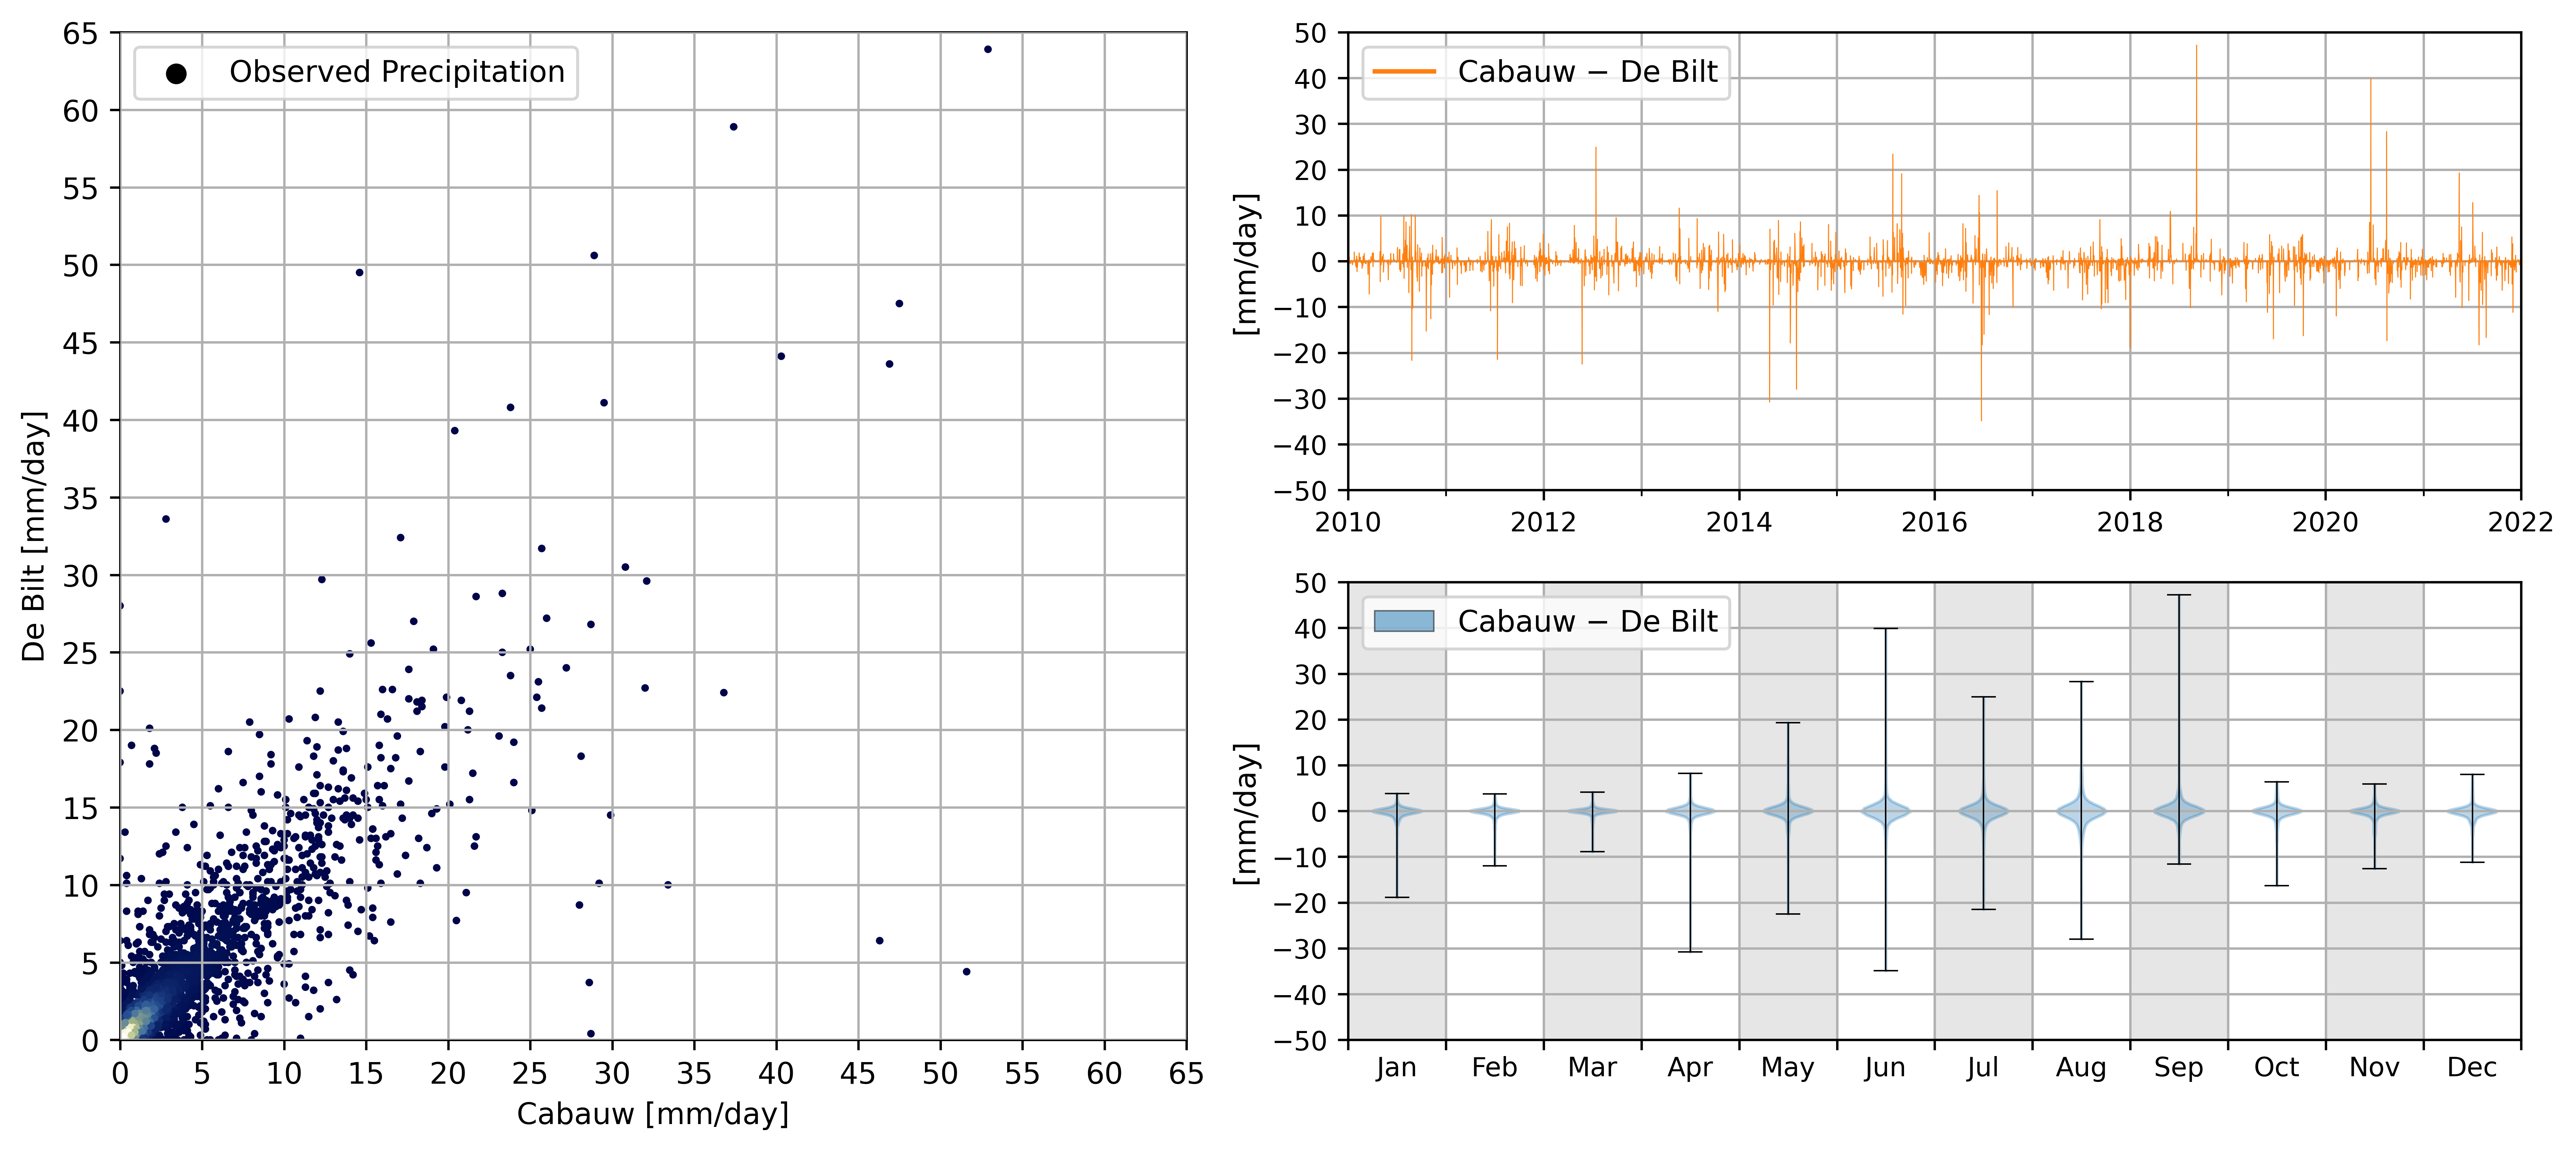
\includegraphics[width=12.0in, height=5.3in, keepaspectratio]{fig/precipitation_compare.png}
\end{tikzfigure}
\vspace{-5mm}
}

\column{0.6}
\block[bodyoffsety=15mm, titleoffsety=15mm, bodyverticalshift=-3mm]{\textsf{Pastas time series models}}
{
\vspace{-1mm}
\begin{minipage}{0.7\linewidth}
    The Python package Pastas \citep{Pastas} uses predefined impulse responses to estimate the contribution of stresses to the hydraulic head fluctuations \citep{Asmuth2002}. An important stress is the groundwater recharge, which can sometimes be estimated using a linear recharge model. The linear recharge model estimates the recharge as a linear combination of the precipitation and potential evaporation mutliplied with a scale factor $f$ (eq. \ref{eq:rech}). The time series model estimates both the recharge flux and the response of the groundwater table to the recharge. Different response functions can be applicable but in general the Gamma response function (eq. \ref{eq:gamma}) is a versatile function that gives a good fit in many circumstances. 
    Parameters of Pastas models are often estimated with the nonlinear least squares algorithm from SciPy \citep{Scipy}. To obtain an accurate estimate of the parameter uncertainty, a first order autoregressive (AR(1)) noise model is applied on the model residuals: $r(t_i) = u(t_i) + r(t_{i+1})\exp{\left(\frac{-\Delta t_i}{\alpha}\right)}$. This results in one extra parameter $\alpha$ that is estimated along with the other parameters by minimizing the sum of squared innovations $u$. On top of that, the head observations are resampled to a lower frequency (generally 14 days) in order to remove autocorrelation in the innovations and obtain so called \textit{white noise}.
\end{minipage}
\hfill
\begin{minipage}{0.3\linewidth}
    \normalsize{
    \begin{equation} \label{eq:convolution}
        h(t) = \int^t_{-\infty}R(\tau)\vartheta(t-\tau)d\tau + d + r(t)
    \end{equation}
    \vspace{2mm}
    \begin{equation} \label{eq:gamma}
        \vartheta(t) = \frac{A}{a^n\Gamma(n)} t^{n-1}\exp(-t/a),
    \end{equation}
    \vspace{2mm}
    \begin{equation} \label{eq:rech}
        R = P + f E_p
    \end{equation}
    }
    \vspace{-6mm}
    \begin{tikzfigure}[Example Gamma Response]\label{fig:gamma}
        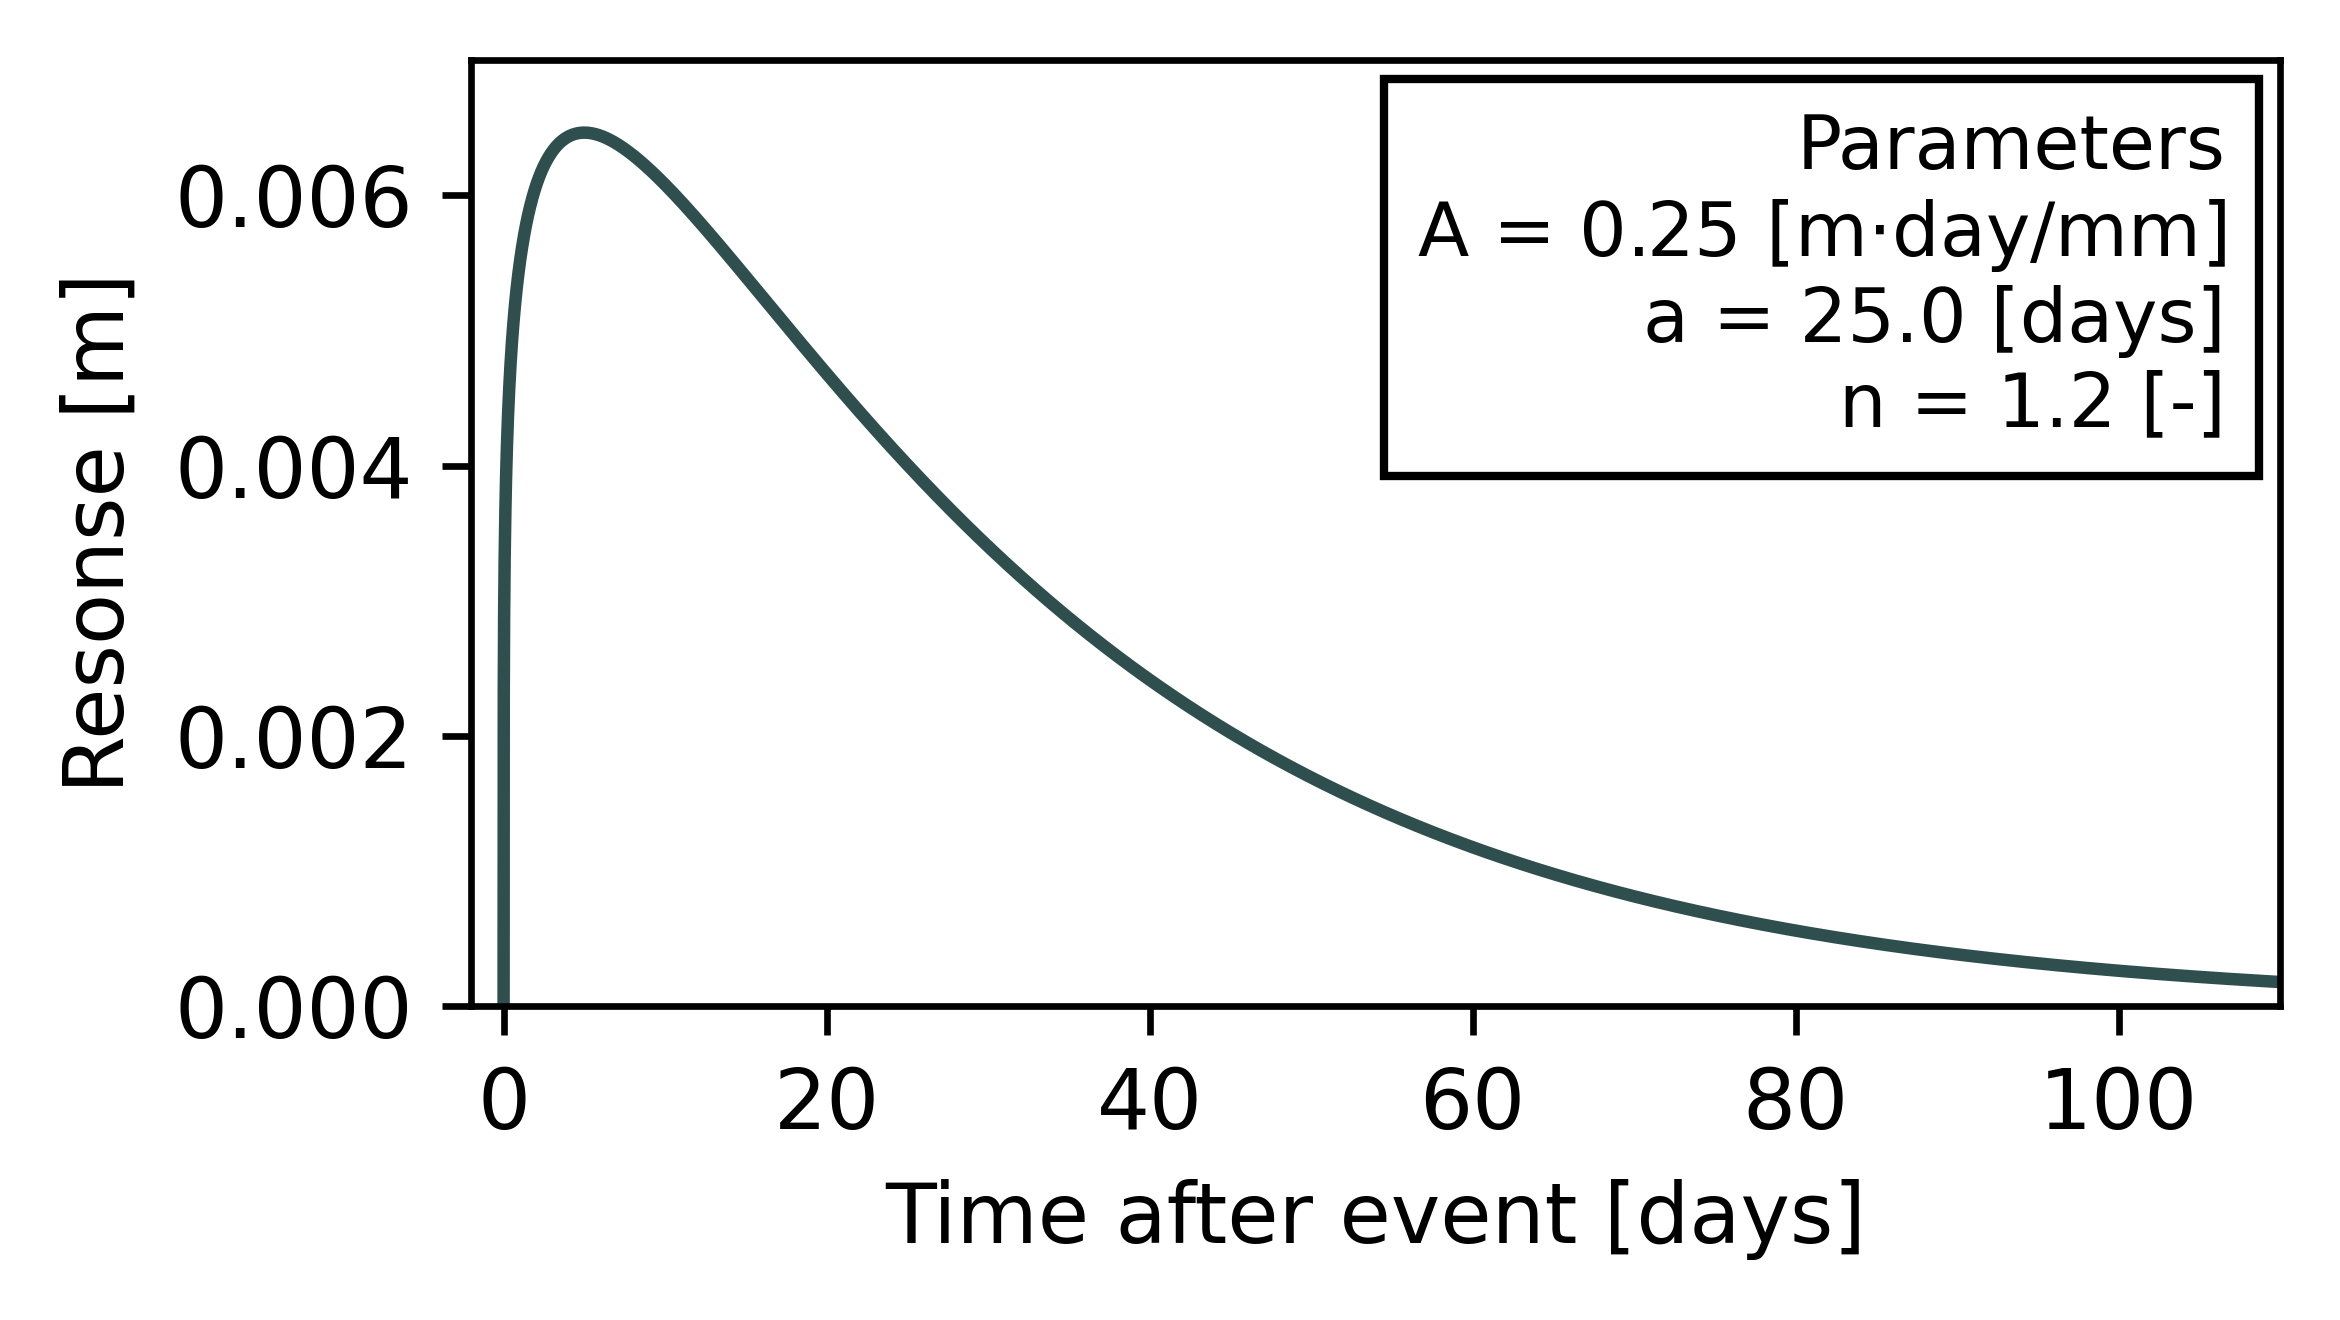
\includegraphics[width=\linewidth, height=60mm, keepaspectratio]{fig/gamma_response.png}
    \end{tikzfigure}
\end{minipage}
\vspace{-5mm}
\begin{tikzfigure}[Input stresses and the simulated head series]\label{fig:meteo_series}
    
\includegraphics[width=18in, height=2.7in, keepaspectratio]{fig/meteo_series.png}
\end{tikzfigure}
\vspace{-12mm}
}

\block[bodyverticalshift=-7mm]{\textsf{Parameter estimation with PEST++ GLM and iES}}
{
\begin{multicols}{2}
    PEST++ uses the Gauss-Levenberg-Marquard (GLM) algorithm to history match model output to observations. pestpp-glm undertakes highly parameterized inversion and is very robust. Parameter uncertainties are calculated via first order, second moment (FOSM) analysis. To fill the jacobian matrix, pestpp-glm runs the model once for each parameter, using a finite difference scheme for the parameter pertubation \citep{White2020}.
    With the iterative ensemble smoothing (iES) approach, ensembles of parameter values and simulation results are used to approximate the jacobian matrix \citep{White2018}. pestpp-ies allows for the expression of uncertainty from the parameter ensembles that each follow their own optimiziation trajectory \citep{Fienen2024}. 
    Recent developments \citep[e.g.][]{GroundwaterModelingChallenge2024} allowed the use of PEST++ (iES) with Pastas. To obtain a prior parameter distribution, the model is solved using SciPy LeastSquares, after which the minimum and maximum parameter bounds are adjusted accordingly. The prior is then constructed from a diagonal prior parameter covariance matrix assuming parameter bounds approximate the range of 95\% confidence.
\end{multicols}
\vspace{-4mm}
}
\end{columns}

\begin{columns}
\column{0.35}
\block[bodyverticalshift=-5mm]{\textsf{Solving with PEST++ GLM examples}}{
\begin{minipage}{\linewidth}
    Correlation coefficients of the parameters from SciPy LeastSquares+AR(1) (upper triangle) and pestpp-glm (lower triangle) FOSM-approximate posterior covariance matrix.\\
    \normalsize{
    \begin{minipage}{0.48\linewidth}
        \begin{tikztable}[Cabauw without Noise]\label{tab:nonoise_cabauw_corr}
            \begin{tabular}{lccccc}
\toprule
 & $A$ & $n$ & $a$ & $f$ & $d$ \\
\midrule
$A$ & {\cellcolor[HTML]{2C1A4C}} \color[HTML]{F1F1F1} 1.00 & {\cellcolor[HTML]{A1A167}} \color[HTML]{F1F1F1} -0.47 & {\cellcolor[HTML]{29396C}} \color[HTML]{F1F1F1} 0.84 & {\cellcolor[HTML]{28477A}} \color[HTML]{F1F1F1} 0.77 & {\cellcolor[HTML]{525224}} \color[HTML]{F1F1F1} -0.79 \\
$n$ & {\cellcolor[HTML]{D7D7AE}} \color[HTML]{000000} -0.23 & {\cellcolor[HTML]{2C1A4C}} \color[HTML]{F1F1F1} 1.00 & {\cellcolor[HTML]{4C4C20}} \color[HTML]{F1F1F1} -0.81 & {\cellcolor[HTML]{CBCB99}} \color[HTML]{000000} -0.30 & {\cellcolor[HTML]{8BA7C2}} \color[HTML]{F1F1F1} 0.33 \\
$a$ & {\cellcolor[HTML]{47729E}} \color[HTML]{F1F1F1} 0.57 & {\cellcolor[HTML]{59592A}} \color[HTML]{F1F1F1} -0.76 & {\cellcolor[HTML]{2C1A4C}} \color[HTML]{F1F1F1} 1.00 & {\cellcolor[HTML]{45719C}} \color[HTML]{F1F1F1} 0.57 & {\cellcolor[HTML]{7D7D48}} \color[HTML]{F1F1F1} -0.61 \\
$f$ & {\cellcolor[HTML]{2C5586}} \color[HTML]{F1F1F1} 0.70 & {\cellcolor[HTML]{EDEEDF}} \color[HTML]{000000} -0.07 & {\cellcolor[HTML]{94AEC7}} \color[HTML]{F1F1F1} 0.30 & {\cellcolor[HTML]{2C1A4C}} \color[HTML]{F1F1F1} 1.00 & {\cellcolor[HTML]{393911}} \color[HTML]{F1F1F1} -0.90 \\
$d$ & {\cellcolor[HTML]{9F9F65}} \color[HTML]{F1F1F1} -0.48 & {\cellcolor[HTML]{C5C58F}} \color[HTML]{000000} -0.33 & {\cellcolor[HTML]{B3C5D7}} \color[HTML]{000000} 0.20 & {\cellcolor[HTML]{555527}} \color[HTML]{F1F1F1} -0.78 & {\cellcolor[HTML]{2C1A4C}} \color[HTML]{F1F1F1} 1.00 \\
\bottomrule
\end{tabular}

        \end{tikztable}
    \end{minipage}
    \hfill
    \begin{minipage}{0.48\linewidth}
        \begin{tikztable}[Cabauw with Noise]\label{tab:noise_cabauw_corr}
            \begin{tabular}{lccccc}
\toprule
 & $A$ & $n$ & $a$ & $f$ & $d$ \\
\midrule
$A$ & {\cellcolor[HTML]{2C1A4C}} \color[HTML]{F1F1F1} 1.00 & {\cellcolor[HTML]{C1C18A}} \color[HTML]{000000} -0.35 & {\cellcolor[HTML]{346191}} \color[HTML]{F1F1F1} 0.65 & {\cellcolor[HTML]{29386A}} \color[HTML]{F1F1F1} 0.84 & {\cellcolor[HTML]{3C3D14}} \color[HTML]{F1F1F1} -0.88 \\
$n$ & {\cellcolor[HTML]{D7D7AE}} \color[HTML]{000000} -0.23 & {\cellcolor[HTML]{2C1A4C}} \color[HTML]{F1F1F1} 1.00 & {\cellcolor[HTML]{434319}} \color[HTML]{F1F1F1} -0.85 & {\cellcolor[HTML]{DEDEBD}} \color[HTML]{000000} -0.19 & {\cellcolor[HTML]{AABED2}} \color[HTML]{000000} 0.23 \\
$a$ & {\cellcolor[HTML]{45719C}} \color[HTML]{F1F1F1} 0.57 & {\cellcolor[HTML]{59592A}} \color[HTML]{F1F1F1} -0.76 & {\cellcolor[HTML]{2C1A4C}} \color[HTML]{F1F1F1} 1.00 & {\cellcolor[HTML]{688CB0}} \color[HTML]{F1F1F1} 0.45 & {\cellcolor[HTML]{999960}} \color[HTML]{F1F1F1} -0.50 \\
$f$ & {\cellcolor[HTML]{2C5586}} \color[HTML]{F1F1F1} 0.70 & {\cellcolor[HTML]{EDEEDF}} \color[HTML]{000000} -0.06 & {\cellcolor[HTML]{92ACC6}} \color[HTML]{F1F1F1} 0.30 & {\cellcolor[HTML]{2C1A4C}} \color[HTML]{F1F1F1} 1.00 & {\cellcolor[HTML]{2E2E08}} \color[HTML]{F1F1F1} -0.96 \\
$d$ & {\cellcolor[HTML]{9D9D63}} \color[HTML]{F1F1F1} -0.49 & {\cellcolor[HTML]{C5C58F}} \color[HTML]{000000} -0.33 & {\cellcolor[HTML]{B3C5D7}} \color[HTML]{000000} 0.20 & {\cellcolor[HTML]{555527}} \color[HTML]{F1F1F1} -0.78 & {\cellcolor[HTML]{2C1A4C}} \color[HTML]{F1F1F1} 1.00 \\
\bottomrule
\end{tabular}

        \end{tikztable}
    \end{minipage}
    \\
    \begin{minipage}{0.48\linewidth}
        \begin{tikztable}[De Bilt without Noise]\label{tab:nonoise_bilt_corr}
            \begin{tabular}{lccccc}
\toprule
 & $A$ & $n$ & $a$ & $f$ & $d$ \\
\midrule
$A$ & {\cellcolor[HTML]{2C1A4C}} \color[HTML]{F1F1F1} 1.00 & {\cellcolor[HTML]{A3A369}} \color[HTML]{F1F1F1} -0.47 & {\cellcolor[HTML]{293B6D}} \color[HTML]{F1F1F1} 0.83 & {\cellcolor[HTML]{283F72}} \color[HTML]{F1F1F1} 0.80 & {\cellcolor[HTML]{4E4E21}} \color[HTML]{F1F1F1} -0.81 \\
$n$ & {\cellcolor[HTML]{D9D9B3}} \color[HTML]{000000} -0.22 & {\cellcolor[HTML]{2C1A4C}} \color[HTML]{F1F1F1} 1.00 & {\cellcolor[HTML]{4C4C20}} \color[HTML]{F1F1F1} -0.82 & {\cellcolor[HTML]{C9C996}} \color[HTML]{000000} -0.31 & {\cellcolor[HTML]{8BA7C2}} \color[HTML]{F1F1F1} 0.33 \\
$a$ & {\cellcolor[HTML]{4D78A1}} \color[HTML]{F1F1F1} 0.55 & {\cellcolor[HTML]{5B5B2C}} \color[HTML]{F1F1F1} -0.75 & {\cellcolor[HTML]{2C1A4C}} \color[HTML]{F1F1F1} 1.00 & {\cellcolor[HTML]{3F6B99}} \color[HTML]{F1F1F1} 0.60 & {\cellcolor[HTML]{7B7B47}} \color[HTML]{F1F1F1} -0.62 \\
$f$ & {\cellcolor[HTML]{2B5385}} \color[HTML]{F1F1F1} 0.70 & {\cellcolor[HTML]{EDEEDF}} \color[HTML]{000000} -0.07 & {\cellcolor[HTML]{97B0C8}} \color[HTML]{000000} 0.29 & {\cellcolor[HTML]{2C1A4C}} \color[HTML]{F1F1F1} 1.00 & {\cellcolor[HTML]{36360F}} \color[HTML]{F1F1F1} -0.92 \\
$d$ & {\cellcolor[HTML]{AAAA6F}} \color[HTML]{F1F1F1} -0.44 & {\cellcolor[HTML]{BCBC83}} \color[HTML]{000000} -0.37 & {\cellcolor[HTML]{9BB3CB}} \color[HTML]{000000} 0.28 & {\cellcolor[HTML]{5F5F2F}} \color[HTML]{F1F1F1} -0.74 & {\cellcolor[HTML]{2C1A4C}} \color[HTML]{F1F1F1} 1.00 \\
\bottomrule
\end{tabular}

        \end{tikztable}
    \end{minipage}
    \hfill
    \begin{minipage}{0.48\linewidth}
        \begin{tikztable}[De Bilt with Noise]\label{tab:noise_bilt_corr}
            \begin{tabular}{lccccc}
\toprule
 & $A$ & $n$ & $a$ & $f$ & $d$ \\
\midrule
$A$ & {\cellcolor[HTML]{2C1A4C}} \color[HTML]{F1F1F1} 1.00 & {\cellcolor[HTML]{B0B075}} \color[HTML]{000000} -0.42 & {\cellcolor[HTML]{284375}} \color[HTML]{F1F1F1} 0.78 & {\cellcolor[HTML]{29386A}} \color[HTML]{F1F1F1} 0.84 & {\cellcolor[HTML]{404016}} \color[HTML]{F1F1F1} -0.87 \\
$n$ & {\cellcolor[HTML]{D8D8B1}} \color[HTML]{000000} -0.22 & {\cellcolor[HTML]{2C1A4C}} \color[HTML]{F1F1F1} 1.00 & {\cellcolor[HTML]{4C4C20}} \color[HTML]{F1F1F1} -0.82 & {\cellcolor[HTML]{CCCC9B}} \color[HTML]{000000} -0.29 & {\cellcolor[HTML]{90AAC5}} \color[HTML]{F1F1F1} 0.32 \\
$a$ & {\cellcolor[HTML]{4B76A0}} \color[HTML]{F1F1F1} 0.55 & {\cellcolor[HTML]{5B5B2C}} \color[HTML]{F1F1F1} -0.75 & {\cellcolor[HTML]{2C1A4C}} \color[HTML]{F1F1F1} 1.00 & {\cellcolor[HTML]{3F6B99}} \color[HTML]{F1F1F1} 0.60 & {\cellcolor[HTML]{777744}} \color[HTML]{F1F1F1} -0.63 \\
$f$ & {\cellcolor[HTML]{2C5586}} \color[HTML]{F1F1F1} 0.70 & {\cellcolor[HTML]{EDEEDF}} \color[HTML]{000000} -0.07 & {\cellcolor[HTML]{97B0C8}} \color[HTML]{000000} 0.30 & {\cellcolor[HTML]{2C1A4C}} \color[HTML]{F1F1F1} 1.00 & {\cellcolor[HTML]{2F300A}} \color[HTML]{F1F1F1} -0.95 \\
$d$ & {\cellcolor[HTML]{A6A66B}} \color[HTML]{F1F1F1} -0.46 & {\cellcolor[HTML]{BEBE85}} \color[HTML]{000000} -0.36 & {\cellcolor[HTML]{A2B9CE}} \color[HTML]{000000} 0.26 & {\cellcolor[HTML]{5D5D2D}} \color[HTML]{F1F1F1} -0.75 & {\cellcolor[HTML]{2C1A4C}} \color[HTML]{F1F1F1} 1.00 \\
\bottomrule
\end{tabular}

        \end{tikztable}
    \end{minipage}
    }
\end{minipage}
}

\column{0.65}
\block[bodyverticalshift=-5mm]{\textsf{Solving with PEST++ iES example}}{
\vspace{-3mm}
\begin{minipage}{0.32\linewidth}
    The pestpp-ies algorithm runs 1000 ensembles with the prior parameters sampled within the provided parameter bounds. Ensembles with a bad fit, approximately 2.5\%, are discarded. A total of 25 iterations is allowed to calculate a posterior distribution but less iterations are allowed if the objective function does not change much anymore between iterations. Noise with a standard deviation of 5 cm is added to the head observations to account for measurement error and model discrepancy \citep{Fienen2024}. The prior and posterior parameter ensembles, including the base realization and true parameter are shown in the upper row of figure \ref{fig:parameter_ensemble}. The lower row shows the 95\% confidence interval of the parameter ensemble for each iteration.
\end{minipage}
\hfill
\begin{minipage}{0.66\linewidth}
     \begin{tikzfigure}[PEST++ iES prior and posterior parameter ensembles (upper row) with the base realization (red) and true parameter value (black dashed) and the 95\% confidence interval per iteration based on the quantiles.] \label{fig:parameter_ensemble}
        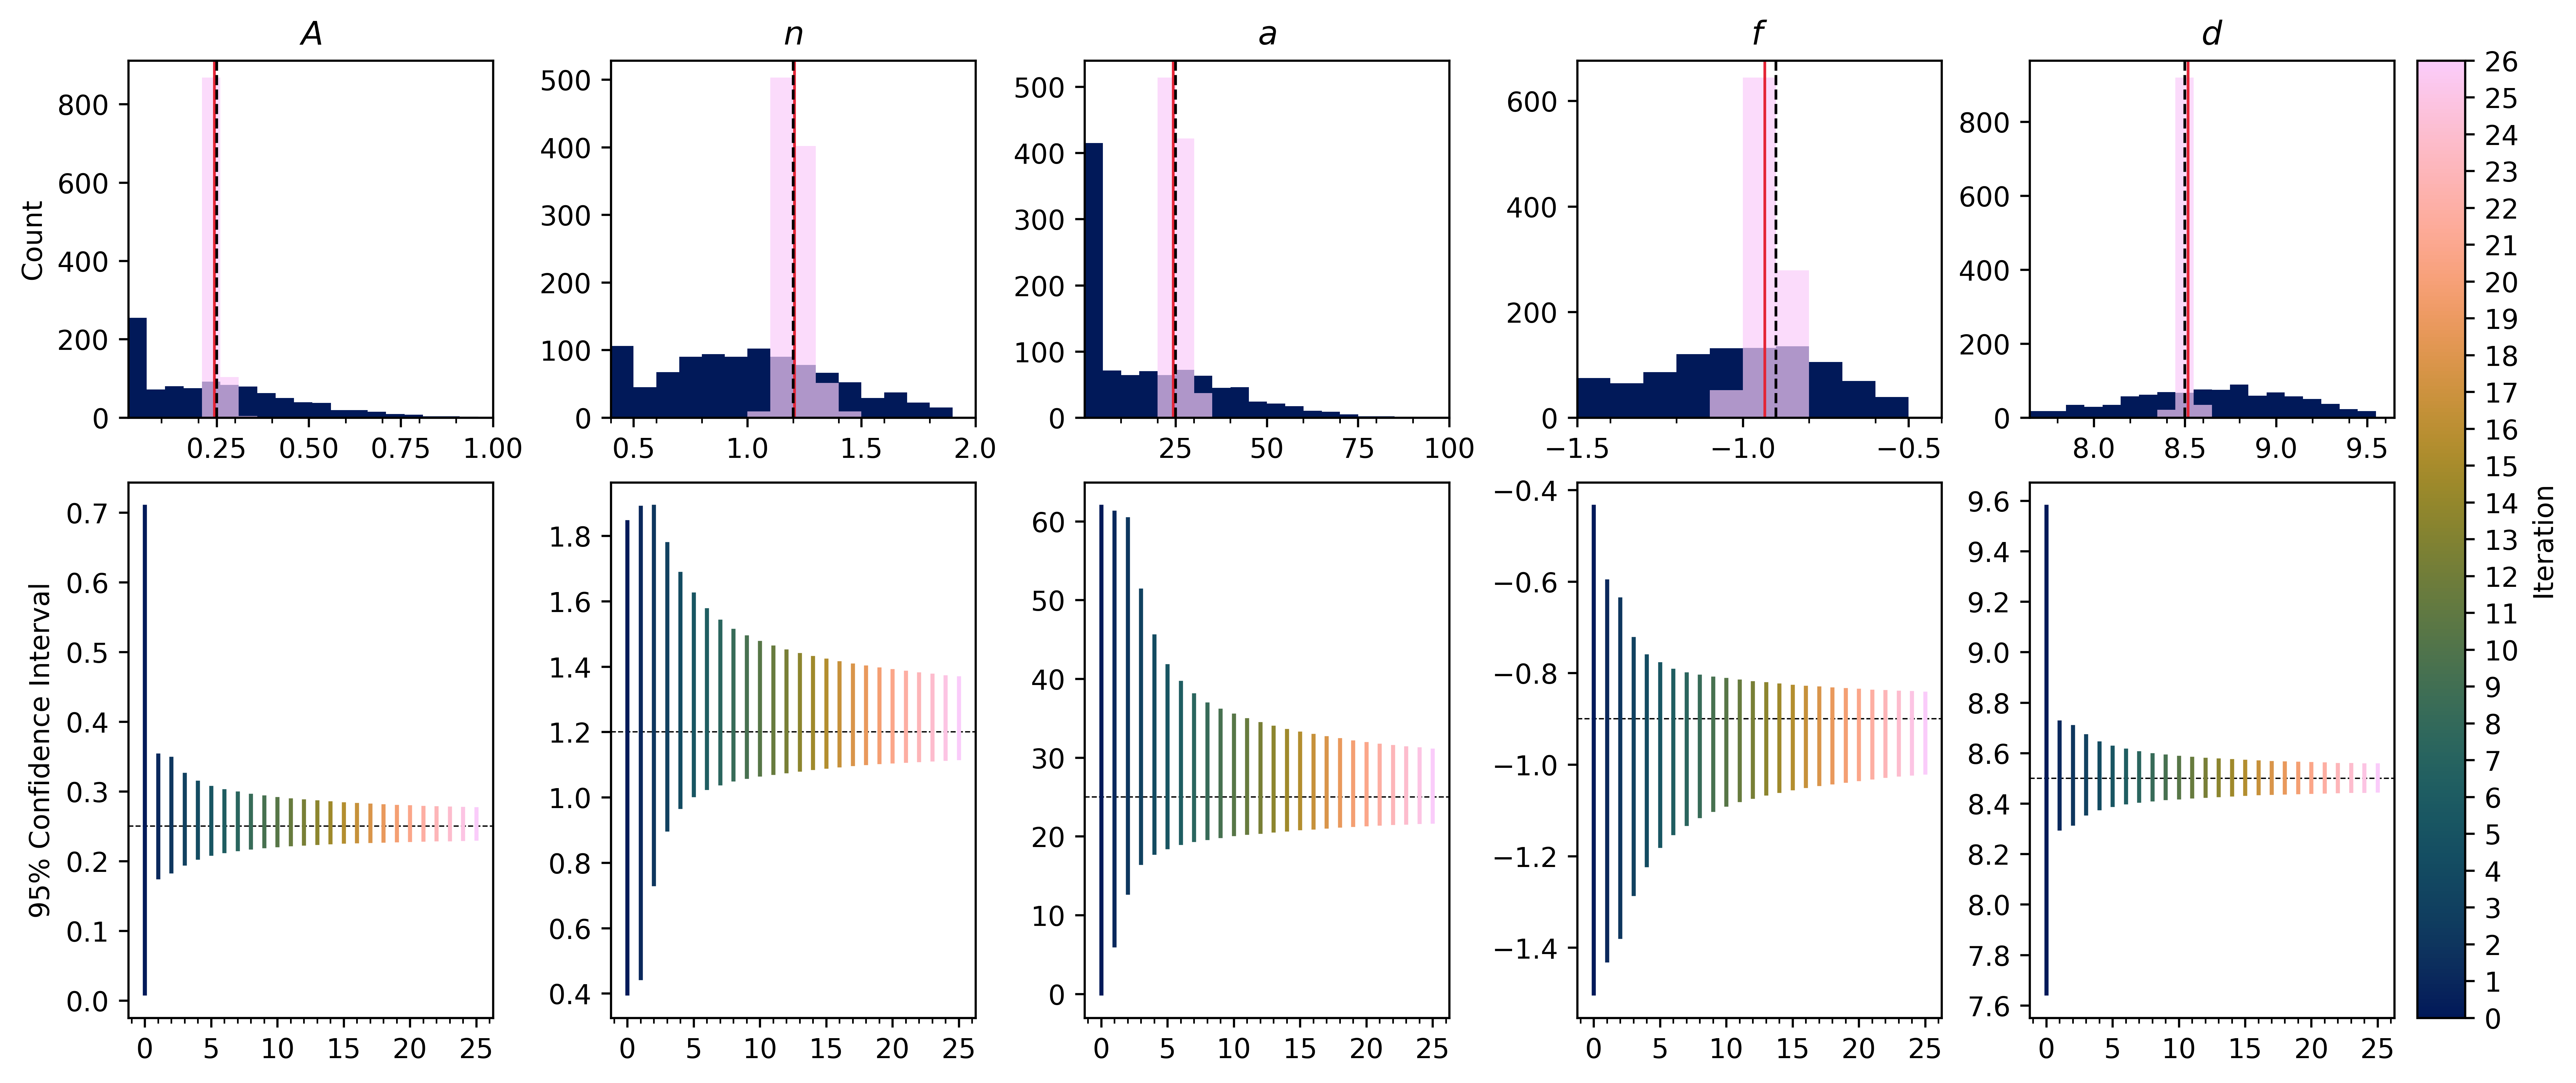
\includegraphics[width=13.0in, height=5.4in]{fig/ensemble_plots/noise_cabauw_pastas_ensemblepar.png}
    \end{tikzfigure}
\end{minipage}
}
\vspace{-13mm}
\end{columns}

\begin{columns}
\column{0.78}
{\block[bodyverticalshift=-8mm]{\textsf{Comparing parameter estimates}}
{
\vspace{-5mm}
\begin{tikzfigure}[Simulation results for scenario 2, Pastas' synthetic head series with noise on the observations and the original precipitation series from Cabauw]\label{fig:simulation_ensemble}
    \includegraphics[width=25.0in, height=6.5in,  keepaspectratio]{fig/ensemble_plots/noise_cabauw_pastas_ensemblesim.png}
\end{tikzfigure}

\begin{minipage}{0.47\linewidth}
    Four scenarios are tested where the parameters are estimated with SciPy+AR(1), pestpp-glm and pestpp-ies:
    \begin{enumerate}
        \item No noise on the head observations and the original precipitation series from Cabauw
        \item Noise on the head observations and the original precipitation series from Cabauw (figures \ref{fig:parameter_ensemble} and \ref{fig:simulation_ensemble})
        \item No noise on head the observations and the precipitation series from De Bilt
        \item Noise on the head observations and the precipitation series from De Bilt
    \end{enumerate}
    The synthetic head time series from figure \ref{fig:meteo_series} with a 14 day frequency is used for a period of twenty years, 2003 through 2022. If noise is added on the head observations, pestpp-glm and SciPy LeastSquares+AR(1) solve only for one noise realization while pestpp-ies has a noise realization for each ensemble. 
\end{minipage}
\hfill
\begin{minipage}{0.52\linewidth}
    \begin{tikzfigure}[Parameter estimates and the 95\% confidence interval. Black dashed lines are the true parameter values.]\label{fig:par_est_pastas}
    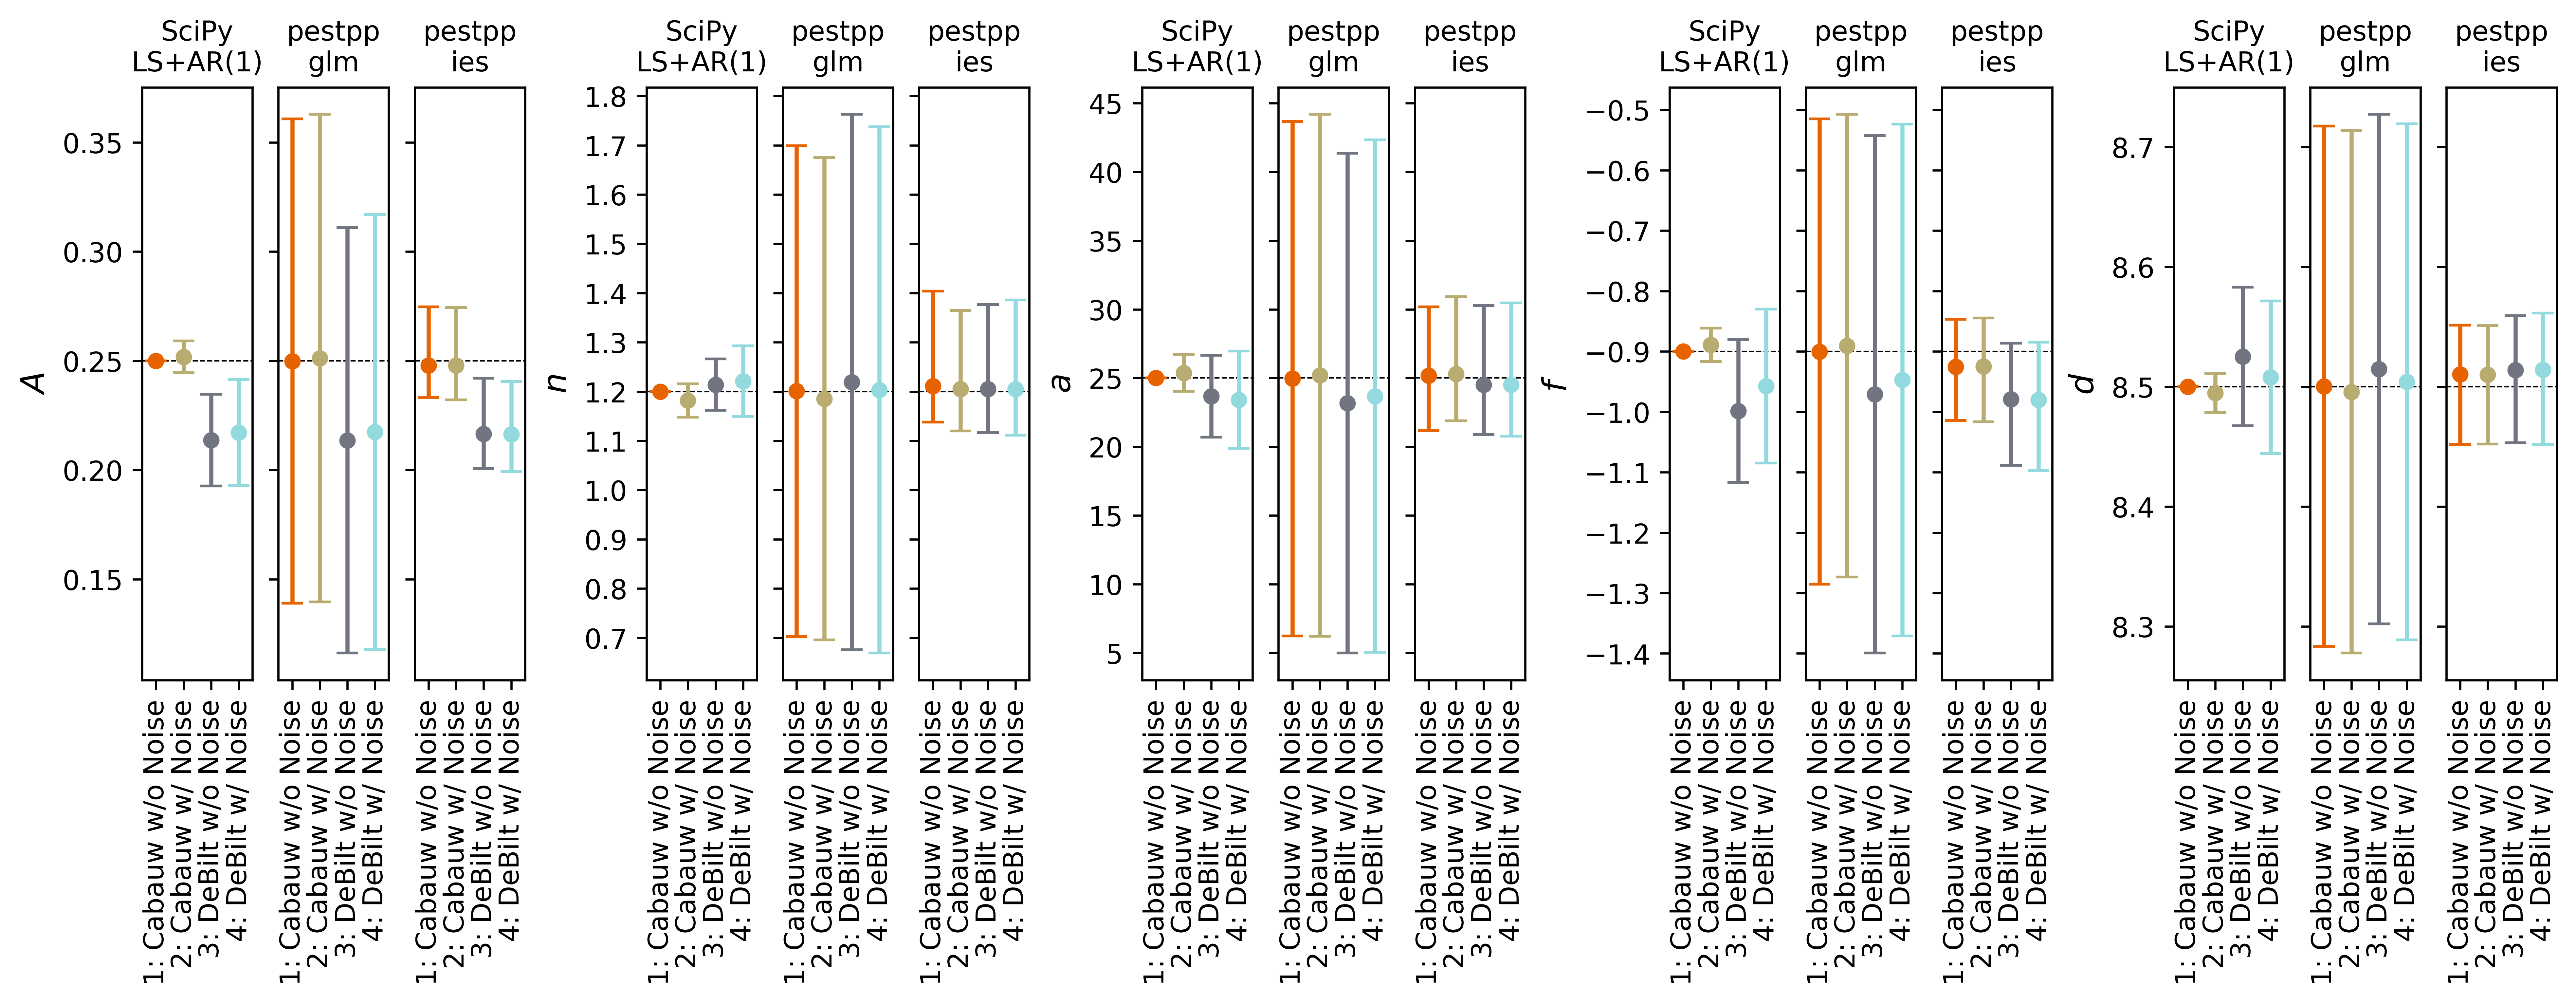
\includegraphics[width=13.0in, height=5.0in]{fig/parameter_estimations_pastas.png}
    \end{tikzfigure}
\end{minipage}
}

\block[bodyverticalshift=-7mm]{\textsf{Testing with realistic synthetic head series}}
{
\begin{minipage}{0.15\linewidth}
    \begin{tikzfigure}[Homogeneous aquifer between two parallel canals]\label{fig:perceel}
        \vspace{-2mm}
        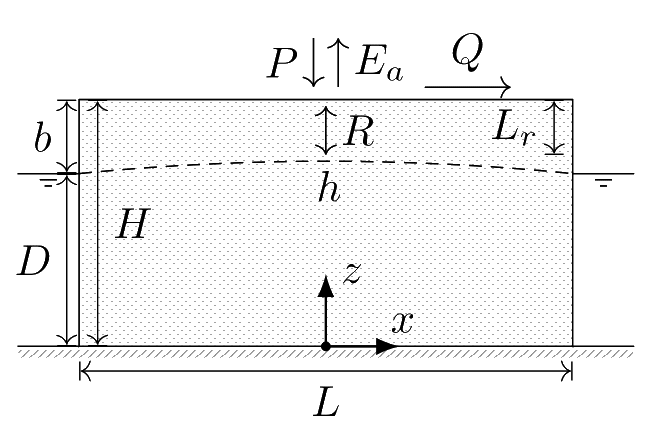
\includegraphics[width=\textwidth, height=3.5in, keepaspectratio]{fig/tikz_perceel.png}
    \end{tikzfigure}
\end{minipage}
\hfill
\begin{minipage}{0.7\linewidth}
    \begin{multicols}{2}
        It can be helpfull to know the true Pastas parameters when analyzing synthetic head series as showed in this poster. However, it might be more usefull to create realistic synthetic head series where physical processes that are deemed important are incorporated. MODFLOW USG-Transport \citep{MFUSG} is an example of a groundwater model used that can be used to generate realistic synthetic heads \citep{Vonk2024}. It numerically solves Richards' equation for two- (and three-) dimensional flow in variably saturated porous media. The van Genuchten soil water retention curve, combined with Brooks-Corey's relative permeability function are used to define the soil hydraulic properties which results in remarkable numerical stability. Due to unsaturated zone processes the head response top precipitation can be higly nonlinear which has been tested for a homogeneous aquifer as seen in figure \ref{fig:perceel}. Read more on this topic in Vonk et al. \citep{Vonk2024} by scanning the QR code!
    \end{multicols}
\end{minipage}
\hfill
\begin{minipage}{0.12\linewidth}
    \begin{tikzfigure}\label{fig:qrcode}
        \centering
        
\includegraphics[width=\textwidth, height=3.5in, keepaspectratio]{fig/bitly_vonk2024.png}
\end{tikzfigure}
\end{minipage}
\vspace{-11mm}
}
}

\column{0.22}
\block[bodyverticalshift=-8mm]{\textsf{Discussion$_{}$}}{
\begin{itemize}[leftmargin=.1in]
    \item Please note that the results on this poster are \textbf{preliminary}! We have more questions than answers at the moment.
    \item Possibilities for interaction between PEST++ and SciPy LeastSquares. SciPy calculates a jacobian for Pastas much faster than PEST++ after which the jacobian can be parsed to PEST++ as prior for iES or posterior to GLM for FOSM(-based Monte Carlo). 
    \item Many opportunities possible within the PEST++ framework for uncertainty estimation. Further exploration of the applicability of PEST++ on time series models is a topic for future research. For instance, PEST++ iES deals efficiently with large parameter samples. This allows for parameterization of the input stresses, i.e., estimating the precipitation error each day.
\end{itemize}
\vspace{-9mm}
}
\block[bodyverticalshift=-30mm]{\textsf{References}}{
\footnotesize
\innerblock{
Contact\\\vspace{5mm}Download}{
m.vonk@artesia-water.nl\\
\\
Download poster as pdf: https://bit.ly/IAH2024
}

\begingroup
\renewcommand{\section}[2]{}%
% \scriptsize
\footnotesize
\bibliography{references.bib}
\endgroup
\vspace{-3mm}
}
\end{columns}

\end{document}